% !TeX spellcheck = nl_NL
\documentclass{article}

\begin{document}
	\subsection{Een generieke pagina voorzien van data} 
	\subsubsection{Wat is het?}
    Voor sommige modellen is de vorige techniek niet haalbaar omwille van het feit dat dit zou resulteren in het genereren van een te groot aantal pagina's. Voor deze modellen is er een andere techniek beschikbaar, \'e\'en pagina (al dan niet per taal) voorzien die we op het laatste moment gaan parsen met de bijhorende data. Ter illustratie beschouwen we de producten, dit kunnen er tienduizenden zijn waardoor de techniek van het genereren uitgesloten wordt (wegens de vermelde nadelen). In plaats daarvan gaan we een generieke pagina aanmaken die we voorzien met de productdata op het moment dat een gebruiker deze opvraagt. 
	\subsubsection{Hoe werkt het?}
    Als eerste hebben we een SlingFilter nodig, deze bekijkt alle binnenkomende request en manipuleert deze indien nodig. Om deze filter te maken voorzien we een Java-klasse van de annotatie in Figuur \ref{fig:sling-filter} en laten deze klasse de javax.servlet.Filter interface implementeren. De meegegeven scope vertelt Sling waar deze filter op werkt, in deze situatie willen we dat elk binnenkomend request deze filter passeert. De order propertie geeft aan in welke volgorde de filters moeten uitgevoerd worden indien er meerdere zijn. Hoe lager dit getal hoe eerder de filter aan bod komt.
    
    \begin{figure}[h!]
  		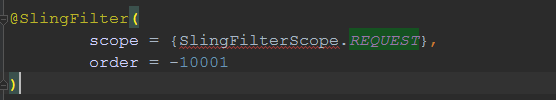
\includegraphics[width=0.8\textwidth]{images/sling-filter.PNG}
  		\label{fig:sling-filter}
	\end{figure}
	
    De Filter interface dwingt ons om drie methoden te implementeren, de init methode wordt uitgevoerd wanneer de filter in gebruik wordt genomen. De destroy methode is actief wanneer een filter wordt opgekuist, hierin kan men eventuele threads afsluiten of resources vrijgeven. Deze twee methodes laten we leeg en we focussen ons op de derde, de doFilter methode. Deze gaat elk binnenkomend request onder de loep nemen en deze (indien gewenst) manipuleren. Voor onze producten gaan we de url van een request bekijken, indien deze het patroon "/product/" bevat, weten we dat deze naar een product pagina moet leiden. We onderscheppen deze requests en sturen deze door naar de generieke product pagina. Voor het redirecten gebeurt gaan we eerst het product ID uit de url halen. Dit ID gebruiken we om (via een REST call) het bijhorende product op te halen en toe te voegen aan het binnengekomen request.
    \par
    De volgende stap is het voorzien van de generieke pagina, dit gebeurt grotendeels conform aan wat we al hebben gezien. We voorzien een HTML met daarop enkele componenten die gebruik maakt van een controller klasse. Het verschil met het reeds geziene is de soort controller dat we gebruiken, voorheen luisterde deze naar een node maar die hebben we deze keer niet. In plaats daarvan willen we de request beschikbaar stellen, daarop staat immers onze product informatie. Om hieraan te kunnen, voorzien we onze controller met de annotatie uit Figuur \ref{fig:request-controller}.

    \begin{figure}[h!]
  		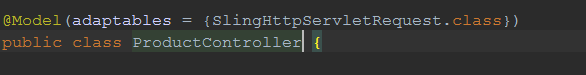
\includegraphics[width=0.8\textwidth]{images/request-controller.PNG}
  		\label{fig:request-controller}
	\end{figure}
    
    Het verschil met een controller voor een node zit in de "adaptables" waarde, voorheen was dit een resource. Door deze waarde te wijzigen weet Sling dat deze controller naar een request moet luisteren. Nu kunnen we via de "@Self" annotatie ons SlingHttpServletRequest ter beschikking stellen. Via de getAttribute methode kunnen we het product opvragen en gaan gebruiken voor bv. de getTitle methode van onze controlleren. 
	\subsubsection{De voordelen}
    Binnen AEM hoeven we maar \'e\'en product pagina te voorzien voor alle producten, in tegenstelling tot het genereren van pagina's. Dit zorgt dat deze techniek de author niet belast. Wanneer een product wijzigt gebeurt er niets totdat diens pagina wordt opgevraagd. Zelfs het opvragen veroorzaakt geen load op de author, het ophalen van de product date en het parsen van de HTML valt onder de verantwoordelijkheid van de publisher.
	\subsubsection{De nadelen}
    Het nadeel is dat deze techniek het moeilijker maakt om gepersonaliseerde product pagina's te voorzien. Een wijziging van de layout op de generieke pagina heeft een rechtstreeks effect op alle producten die deze gebruiken. Men kan hier rond werken door meerdere generieke pagina's te voorzien en op basis van het product naar een specifieke te redirecten. Zo kan men groepen van producten een ander uitzicht geven.
    \par
    Een ander (miniem) nadeel is de afhankelijkheid van REST services, als deze falen kan de data niet worden opgehaald en bijgevolg de pagina niet getoond worden. In deze proef ligt het beheer van deze services bij ons en zal downtime onwaarschijnlijk zijn. Wanneer men met externe services werkt, kan men beter een fallback inbouwen in het geval dat deze onverwacht offline gaan.
\end{document}